\documentclass[conference]{IEEEtran}
\usepackage{graphicx}
\usepackage{amsmath}
\usepackage{booktabs}
\usepackage{hyperref}
\usepackage{listings}
\usepackage{xcolor}
\usepackage{tikz}
\usetikzlibrary{arrows.meta, positioning}
\usepackage[utf8]{inputenc}
\usepackage[T1]{fontenc}

\lstset{
  basicstyle=\ttfamily\scriptsize,
  breaklines=true,
  frame=single,
  columns=fullflexible,
}

\begin{document}

\title{Retail Vision Intelligence System: \\
Um Sistema Multi-Componente para Inspeção Automática de Prateleiras com LLMs Multimodais}

\author{
\IEEEauthorblockN{Aluno(a)}
\IEEEauthorblockA{Licenciatura em Inteligência Artificial e Ciência de Dados (LIACD) \\
Trabalho Prático \#2 --- Interação com Modelos de Grande Escala \\
Ano letivo 2025/2026}
}

\maketitle

\begin{abstract}
Este relatório descreve a conceção, implementação e avaliação de um sistema de
inteligência de retalho baseado em modelos de grande escala (LLMs)
multimodais, composto por cinco componentes integrados: (1) um inspetor
visual de prateleiras baseado no Gemini, que produz \textit{inspection
records} JSON estruturados; (2) um motor de regras que converte descrições em
linguagem natural em regras executáveis com deteção de ambiguidade; (3) uma
memória semântica (RAG) sobre o histórico de inspeções, com sumarização e
síntese de respostas por LLM; (4) um gerador de relatórios de sessão em
Markdown; e (5) uma interface de linha de comandos conversacional que integra
os restantes componentes segundo a gramática de comandos especificada no
enunciado. O sistema foi construído sobre um conjunto de 500 imagens reais do
dataset público SKU-110K, sem qualquer imagem sintética. Durante o
desenvolvimento foi identificada uma limitação severa e não documentada da
\textit{free tier} da API Gemini --- um limite de 20 pedidos por dia por
modelo por projeto --- que condicionou fortemente a metodologia de avaliação.
Reportam-se resultados honestos para três estratégias de \textit{prompting}
(zero-shot, \textit{chain-of-thought} e \textit{few-shot}), para três
estratégias de \textit{chunking} no RAG (Recall@3, Faithfulness, Answer
Relevance), para o motor de regras (Rule Parse Rate, Rule Correctness,
Ambiguity Detection) e para uma avaliação \textit{LLM-as-judge} de pequena
escala, todas agregadas pelo harness \texttt{evaluate.py}.
\end{abstract}

\section{Introdução e Arquitetura}
\label{sec:intro}

A gestão visual de prateleiras (\textit{shelf auditing}) é uma tarefa
central no retalho, tradicionalmente realizada por inspeção humana
periódica. O surgimento de modelos de visão-linguagem multimodais de uso
geral (como a família Gemini) torna viável a automação parcial desta tarefa
sem necessidade de treinar modelos de visão dedicados, recorrendo apenas a
\textit{prompting} sobre imagens.

Este trabalho implementa um sistema completo, denominado \textit{Retail
Vision Intelligence System}, que cobre todo o ciclo de vida da informação de
inspeção: desde a análise visual de uma imagem (Componente 1), à deteção
automática de violações de regras de negócio definidas em linguagem natural
pelo gestor de loja (Componente 2), à indexação e recuperação semântica do
histórico de inspeções com síntese de respostas (Componente 3), à geração de
relatórios de sessão estruturados (Componente 4), até a uma interface
unificada que orquestra todos os componentes anteriores segundo a gramática
de comandos da Secção 8 do enunciado (Componente 5).

Um objetivo transversal e não negociável deste trabalho foi garantir que
\textbf{nenhuma imagem do conjunto de dados é sintética}: todas as 500
imagens utilizadas são fotografias reais de prateleiras de retalho,
provenientes do dataset público SKU-110K \cite{sku110k}. A Secção
\ref{sec:dataset} descreve em detalhe a metodologia usada para construir,
sob esta restrição, um conjunto de dados balanceado por categorias de
interesse (prateleiras normais, sujas, ambíguas, vazias e com violações de
planograma).

Durante a implementação, surgiu um obstáculo significativo e não previsto: a
\textit{free tier} da API Gemini impõe um limite de \textbf{20 pedidos por
dia, por modelo, por projeto} (\texttt{GenerateRequestsPerDayPerProjectPer\-Model-FreeTier},
\texttt{quotaValue=20}), muito mais restritivo do que o limite de 1500
pedidos/dia inicialmente assumido a partir da documentação geral. Esta
limitação, discutida em detalhe na Secção \ref{sec:quota}, moldou
significativamente a metodologia de avaliação adotada (uso intensivo de
\textit{cache}, redução do número de imagens avaliadas por estratégia,
substituição de modelos, \textit{fallback} determinista para o RAG) e é, em
si, um resultado relevante deste trabalho.

\subsection{Arquitetura do Sistema}

O sistema está organizado em cinco componentes independentes, cada um
implementado como um módulo Python autónomo com a sua própria interface de
linha de comandos, e um harness de avaliação (\texttt{evaluate.py}) que
agrega métricas de todos eles. A Figura~\ref{fig:arquitetura} ilustra o
fluxo de dados entre componentes.

\begin{figure}[h]
\centering
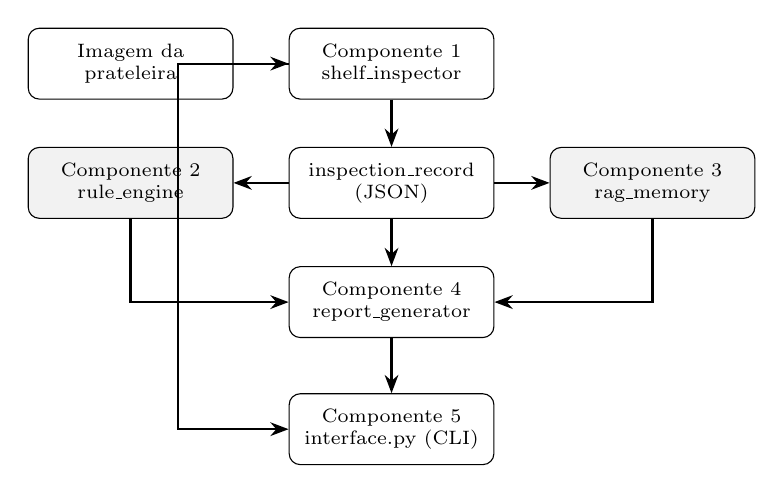
\begin{tikzpicture}[
  box/.style={draw, rounded corners, align=center, minimum width=2.6cm, minimum height=0.9cm, font=\scriptsize},
  arr/.style={-{Stealth}, thick}
]
  \node[box] (img) {Imagem da \\ prateleira};
  \node[box, right=0.7cm of img] (c1) {Componente 1 \\ shelf\_inspector};
  \node[box, below=0.6cm of c1] (record) {inspection\_record \\ (JSON)};
  \node[box, left=0.7cm of record, fill=gray!10] (c2) {Componente 2 \\ rule\_engine};
  \node[box, right=0.7cm of record, fill=gray!10] (c3) {Componente 3 \\ rag\_memory};
  \node[box, below=0.6cm of record] (c4) {Componente 4 \\ report\_generator};
  \node[box, below=0.7cm of c4] (c5) {Componente 5 \\ interface.py (CLI)};

  \draw[arr] (img) -- (c1);
  \draw[arr] (c1) -- (record);
  \draw[arr] (record) -- (c2);
  \draw[arr] (record) -- (c3);
  \draw[arr] (record) -- (c4);
  \draw[arr] (c2) |- (c4);
  \draw[arr] (c3) |- (c4);
  \draw[arr] (c4) -- (c5);
  \draw[arr] (c1.west) -| ([xshift=-1.4cm]c1.west) |- (c5.west);
\end{tikzpicture}
\caption{Fluxo de dados entre os cinco componentes. Uma imagem entra no
Componente 1, que produz um \textit{inspection record} persistido em
\texttt{data/inspections/}. Este record é avaliado pelas regras ativas
(Componente 2), indexado na memória semântica (Componente 3) e usado pelo
Componente 4 para gerar um relatório de sessão que inclui as saídas de (2) e
(3). O Componente 5 expõe todo este fluxo através de uma única CLI com
estado de sessão persistente (\texttt{data/session\_state.json}).}
\label{fig:arquitetura}
\end{figure}

\begin{itemize}
  \item \textbf{\texttt{src/shelf\_inspector.py}} --- recebe uma imagem de
  prateleira e produz um \textit{inspection record} JSON estruturado
  (Secção 4.2 do enunciado), com cache em disco, \textit{rate limiting} e
  \textit{fallback} gracioso.
  \item \textbf{\texttt{src/rule\_engine.py}} --- converte descrições de
  regras de deteção em linguagem natural em regras JSON estruturadas
  (Secção 5.3 do enunciado), com deteção de ambiguidade documentada por
  regra.
  \item \textbf{\texttt{src/rag\_memory.py}} --- indexa o histórico de
  \textit{inspection records} em ChromaDB com \textit{embeddings}
  multilingues, gera resumos por LLM (Secção 6.2) e sintetiza respostas em
  linguagem natural com citação explícita de \texttt{inspection\_id} e data
  (Secção 6.4).
  \item \textbf{\texttt{src/report\_generator.py}} --- gera relatórios de
  sessão em Markdown com seis secções (Secção 7 do enunciado), combinando
  \textit{inspection records}, regras acionadas, contexto histórico do RAG e
  recomendações.
  \item \textbf{\texttt{src/interface.py}} --- interface de linha de
  comandos que implementa a gramática de comandos da Secção 8 do enunciado
  (\texttt{inspect}, \texttt{add rule}, \texttt{list rules},
  \texttt{delete rule}, \texttt{test rule}, \texttt{history},
  \texttt{compare}, \texttt{report}), mantendo um estado de sessão com
  regras carregadas e histórico de inspeções, sem expor \textit{stack
  traces}.
\end{itemize}

\section{Construção do Dataset}
\label{sec:dataset}

\subsection{Restrição de imagens reais}

O requisito mais restritivo deste trabalho foi a proibição total de imagens
geradas sinteticamente para qualquer categoria do dataset. Esta restrição
aplicou-se inclusivamente às categorias mais difíceis de obter num dataset
genérico de deteção de objetos como o SKU-110K: \textit{prateleiras vazias}
e \textit{violações de planograma}, categorias que não existem como
\textit{labels} explícitos no dataset original.

\subsection{Categorização heurística}

Para as categorias \textit{normal}, \textit{dirty} (suja) e
\textit{ambiguous} (ambígua), foi usada uma heurística de \textit{clutter
score} calculada sobre cada imagem candidata:

\begin{equation}
\text{clutter} = 0.7 \cdot \sigma_{\text{edges}} + 0.3 \cdot \sigma_{\text{cor}}
\end{equation}

onde $\sigma_{\text{edges}}$ é o desvio-padrão da imagem após um filtro de
deteção de contornos (\texttt{PIL.ImageFilter.FIND\_EDGES}) sobre uma versão
em escala de cinzentos redimensionada para $256\times256$, e
$\sigma_{\text{cor}}$ é o desvio-padrão dos valores RGB da imagem
redimensionada. Imagens com \textit{clutter score} baixo foram classificadas
como \textit{normal} (prateleiras bem organizadas), valores intermédios como
\textit{ambiguous}, e valores altos como \textit{dirty} (prateleiras
desorganizadas/com muito ruído visual).

\subsection{Categorias \textit{empty} e \textit{planogram\_violation}}

Para estas duas categorias, sem correspondência direta no SKU-110K, foram
combinadas duas estratégias:

\begin{enumerate}
  \item \textbf{Seleção heurística}: aplicando o mesmo \textit{clutter
  score} a um conjunto alargado de imagens candidatas
  (\texttt{data/images/pool\_candidates/}), as imagens com pontuação mais
  baixa (visualmente mais uniformes/menos preenchidas) foram selecionadas
  para \textit{empty}, e as imagens com pontuação mais alta (visualmente
  mais caóticas) para \textit{planogram\_violation}. Este processo está
  implementado em \texttt{scripts/select\_empty\_violation.py} e não envolve
  qualquer chamada a um LLM.
  \item \textbf{Validação por LLM}: para um subconjunto de 6 imagens (4 para
  \textit{empty}, 2 para \textit{planogram\_violation}), o próprio
  Componente 1 (\texttt{shelf\_inspector.py}, estratégia B) foi usado para
  confirmar visualmente, a partir do seu \texttt{model\_reasoning}, que a
  imagem correspondia de facto a uma prateleira com espaços vazios
  significativos ou com produtos visivelmente fora do local esperado. Esta
  proveniência está documentada por imagem na coluna
  \texttt{selection\_method} de \texttt{data/images/manifest.csv}.
\end{enumerate}

É importante notar uma limitação honesta: como a categorização final
assenta em heurísticas de baixo nível (densidade de contornos, variância de
cor) e não em \textit{labels} semânticos, o conteúdo real de algumas imagens
nas pastas \texttt{empty/} e \texttt{ambiguous/} nem sempre corresponde
literalmente ao nome da pasta --- por exemplo, algumas imagens em
\texttt{empty/} mostram prateleiras completamente abastecidas mas
visualmente uniformes. Por este motivo, o \textit{ground truth} usado para
avaliar o Componente 1 (Secção \ref{sec:ground-truth}) foi construído a
partir de inspeção visual humana direta de cada imagem, e não a partir do
nome da pasta de origem.

\subsection{Estatísticas finais do dataset}

A Tabela~\ref{tab:dataset} resume a composição final do dataset, persistida
em \texttt{data/images/manifest.csv} (500 linhas), satisfazendo todos os
mínimos definidos no enunciado.

\begin{table}[h]
\centering
\caption{Composição do dataset (500 imagens, 100\% reais, SKU-110K)}
\label{tab:dataset}
\begin{tabular}{lcc}
\toprule
Categoria & N.º de imagens & Sintética? \\
\midrule
normal & 150 & Não \\
dirty (suja) & 80 & Não \\
ambiguous (ambígua) & 70 & Não \\
empty (vazia) & 100 & Não \\
planogram\_violation & 100 & Não \\
\midrule
\textbf{Total} & \textbf{500} & \textbf{0\% sintéticas} \\
\bottomrule
\end{tabular}
\end{table}

\section{Componente 1: Análise Visual de Prateleiras}
\label{sec:visual}

\subsection{\textit{Schema} de saída e estratégias de \textit{prompting}}

Para cada imagem, o Componente 1 produz um \textit{inspection record} JSON
em conformidade com o \textit{schema} da Secção 4.2 do enunciado:
\texttt{inspection\_id}, \texttt{timestamp}, \texttt{image\_path},
\texttt{zone\_id}, \texttt{overall\_status}
(\texttt{ok}/\texttt{warning}/\texttt{critical}), \texttt{issues} (lista de
problemas com \texttt{issue\_id}, \texttt{type}, \texttt{location},
\texttt{severity}, \texttt{description}, \texttt{confidence} e
\texttt{affected\_area\_pct}), \texttt{shelf\_fill\_rate},
\texttt{products\_detected} e \texttt{model\_reasoning}. Os tipos de
problema considerados são: \texttt{empty\_shelf}, \texttt{wrong\_product},
\texttt{damaged}, \texttt{misaligned}, \texttt{label\_missing} e
\texttt{other}.

Foram implementadas e comparadas três estratégias de \textit{prompting}:

\begin{itemize}
  \item \textbf{A --- Zero-shot}: instrução direta e o \textit{schema} JSON
  pretendido, sem exemplos nem raciocínio intermédio explícito.
  \item \textbf{B --- \textit{Chain-of-thought} (CoT) visual}: o modelo é
  instruído a produzir um \texttt{model\_reasoning} estruturado em quatro
  passos (descrição geral, análise zona-a-zona, identificação de anomalias,
  classificação final) antes/durante a produção do JSON. É a estratégia
  usada por omissão na interface (Componente 5).
  \item \textbf{C --- \textit{Few-shot}}: o prompt inclui exemplos textuais
  de pares (descrição de imagem $\rightarrow$ JSON esperado) antes de pedir
  a análise da imagem real.
\end{itemize}

\subsection{Mecanismos de robustez: \textit{cache}, \textit{rate limiting} e \textit{fallback}}

Dada a limitação de quota descrita na Secção \ref{sec:quota}, o Componente 1
implementa:

\begin{itemize}
  \item \textbf{Cache em disco} (\texttt{cache/}), indexado por
  $\text{MD5}(\text{imagem}) \times \text{estratégia} \times \text{zona}$,
  evitando reanálises desnecessárias da mesma imagem.
  \item \textbf{\textit{Rate limiting}} (RPM configurável, 15 req/min por
  omissão) com \textit{backoff} exponencial em caso de erro 429.
  \item \textbf{\textit{Fallback} gracioso}: quando a quota diária está
  esgotada e não existe entrada em \textit{cache}, o sistema devolve um
  \textit{record} com \texttt{overall\_status="unknown"} e
  \texttt{\_fallback=true}, em vez de falhar --- e a interface (Componente
  5) nunca propaga este erro como \textit{stack trace} ao utilizador.
\end{itemize}

\subsection{Limitação Crítica: Quota da API Gemini \textit{Free Tier}}
\label{sec:quota}

Durante a fase de avaliação, todas as chamadas ao modelo
\texttt{gemini-2.5-flash} começaram a devolver erros HTTP 429 com a
mensagem \texttt{quotaValue: '20'} para a métrica
\texttt{GenerateRequestsPerDayPerProjectPerModel-FreeTier}. Isto contraria a
expectativa inicial (baseada na documentação geral da \textit{free tier}) de
um limite de 1500 pedidos/dia. Investigação adicional confirmou que:

\begin{itemize}
  \item O limite de \textbf{20 pedidos/dia} aplica-se \textit{por modelo, por
  projeto}, e não de forma agregada.
  \item Os modelos \texttt{gemini-2.5-flash}, \texttt{gemini-2.5-flash-lite},
  \texttt{gemini-2.0-flash}, \texttt{gemini-2.0-flash-lite} e
  \texttt{gemini-2.5-pro} esgotaram-se rapidamente durante os testes (cada um
  oferece apenas $\sim$20 pedidos/dia gratuitos).
  \item O modelo \texttt{gemini-3-flash-preview} manteve quota disponível
  durante o desenvolvimento, mas devolve ocasionalmente erros HTTP 503
  (\textit{"model is currently experiencing high demand"}), transitórios.
\end{itemize}

\textbf{Impacto na metodologia}: este limite tornou impraticável re-executar
o Componente 1 sobre as 500 imagens do dataset completo para fins de
avaliação. A estratégia adotada foi:

\begin{enumerate}
  \item Restringir a comparação de estratégias de \textit{prompting}
  (Secção \ref{sec:strategy-comparison}) e a invocação obrigatória de
  \texttt{evaluate.py --images-dir} a um subconjunto de 15 imagens com
  \textit{ground truth} manual.
  \item Para o motor de regras (Componente 2), substituir o modelo por
  \texttt{gemini-3-flash-preview} quando a quota do
  \texttt{gemini-2.5-flash-lite}/\texttt{gemini-2.5-flash} se esgotou a meio
  dos testes.
  \item Para a memória RAG (Componente 3) e o gerador de relatórios
  (Componente 4), usar por omissão resumos gerados localmente
  (\textit{template}) a partir dos campos estruturados dos \textit{records}
  já existentes, reservando as chamadas LLM (resumo e síntese de respostas,
  Secção \ref{sec:rag}) para quando há quota disponível, com \textit{fallback}
  determinista caso contrário.
  \item Para o \textit{LLM-as-judge} (Secção \ref{sec:judge}), reutilizar
  \textit{records} já em \textit{cache} (sem reanalisar imagens) e limitar o
  número de chamadas de avaliação a uma amostra pequena (3 imagens).
\end{enumerate}

Esta limitação é, por si só, um achado relevante para qualquer sistema
real construído sobre a \textit{free tier} da API Gemini: o
dimensionamento de um sistema de produção exigiria obrigatoriamente um
plano pago ou a distribuição de carga por múltiplos modelos/projetos.

\subsection{\textit{Ground truth} e métricas}
\label{sec:ground-truth}
\label{sec:strategy-comparison}

Foi construído um \textit{ground truth} manual
(\texttt{data/ground\_truth.json}) para 15 imagens (3 por categoria do
dataset), com base em inspeção visual humana direta de cada imagem ---
e não nos rótulos de pasta heurísticos ---, registando
\texttt{overall\_status}, \texttt{issues} (tipo, severidade,
\texttt{affected\_area\_pct}), \texttt{shelf\_fill\_rate} e notas
descritivas. No total, o \textit{ground truth} contém 6 ocorrências de
\textit{issues} distribuídas por 3 tipos: \texttt{empty\_shelf} (3),
\texttt{wrong\_product} (2) e \texttt{damaged} (1). Estas mesmas 15 imagens
foram copiadas para \texttt{test\_images/}, usado pela invocação obrigatória
do harness de avaliação (Secção \ref{sec:eval}).

Para cada estratégia $S \in \{A, B, C\}$ e cada imagem, foram calculadas as
métricas da Secção 9.2 do enunciado (\texttt{scripts/compare\_strategies.py}
e \texttt{evaluate.py}): \textbf{API Success Rate}, \textbf{JSON Parse
Rate}, \textbf{Issue Detection Rate} (\textit{recall}), \textbf{False
Positive Rate}, \textbf{Severity Accuracy} e \textbf{Hallucination Rate}
(fração de imagens \texttt{ok} no \textit{ground truth} em que o modelo
reportou pelo menos um problema).

\subsection{Resultados}

A Tabela~\ref{tab:strategies} apresenta os resultados obtidos com
\texttt{gemini-2.5-flash-lite} sobre as 15 imagens de \textit{ground truth}
(\texttt{scripts/compare\_strategies.py}). A Tabela~\ref{tab:imagesdir}
apresenta os resultados da invocação obrigatória
\texttt{evaluate.py --images-dir test\_images/ --output evaluation\_report.json}
com a estratégia B e o modelo \texttt{gemini-2.5-flash}, combinando
\textit{records} já em \textit{cache} com novas chamadas (sujeitas ao
limite de quota da Secção \ref{sec:quota}).

\begin{table}[h]
\centering
\caption{Comparação das estratégias de \textit{prompting} (n=15 imagens, gemini-2.5-flash-lite)}
\label{tab:strategies}
\begin{tabular}{lccc}
\toprule
Métrica & A (zero-shot) & B (CoT) & C (few-shot) \\
\midrule
API success rate & 1.00 & 0.53 & 0.07 \\
JSON parse rate & 0.93 & 1.00 & 1.00 \\
Issue detection rate & 0.00 & 0.00 & 0.00 \\
False positive rate & 0.00 & 0.00 & 0.00 \\
Severity accuracy & N/A & N/A & N/A \\
Hallucination rate & 0.00 & 0.00 & 0.00 \\
\bottomrule
\end{tabular}
\end{table}

\begin{table}[h]
\centering
\caption{\texttt{evaluate.py --images-dir test\_images/} (n=15, estratégia B, gemini-2.5-flash)}
\label{tab:imagesdir}
\begin{tabular}{lc}
\toprule
Métrica & Valor \\
\midrule
API success rate & 0.60 \\
JSON parse rate & 1.00 \\
Issue detection rate & 0.00 \\
False positive rate & 1.00 \\
Severity accuracy & N/A (sem tipos coincidentes) \\
Hallucination rate & 0.10 \\
\bottomrule
\end{tabular}
\end{table}

\subsection{Discussão e análise de casos de falha}

\textbf{1. O custo em \textit{tokens} domina a fiabilidade da API.} Na
Tabela~\ref{tab:strategies}, a estratégia A (prompt e saída mais curtos)
obteve 100\% de sucesso na API, enquanto a estratégia B (CoT, com um campo
\texttt{model\_reasoning} extenso) caiu para 53\%, e a estratégia C
(\textit{few-shot}, com exemplos adicionais no prompt de entrada) caiu para
apenas 7\%. Na Tabela~\ref{tab:imagesdir} (estratégia B, modelo
\texttt{gemini-2.5-flash}, execução mais recente), o \textit{api\_success\_rate}
foi de 0.60 (9/15 imagens), com as restantes 6 a esgotarem todas as
tentativas de \textit{retry} (\textit{backoff} exponencial até 16s,
mensagens \texttt{[429] erro de rate limit}) e a caírem em
\textit{fallback}. Isto sugere fortemente que, além do limite de
pedidos/dia, existe também um limite de \textit{tokens por minuto} (TPM) que
penaliza desproporcionalmente prompts e respostas longas --- um fator
habitualmente menos discutido do que o RPM ou RPD, mas claramente dominante
neste cenário de \textit{free tier}.

\textbf{2. \textit{Issue detection rate} de 0\% --- caso de falha
\texttt{train\_1291.jpg}.} Em ambas as tabelas, \textit{issue detection
rate}\,$=0$. Este resultado foi verificado manualmente lendo os
\textit{records} JSON produzidos: para \texttt{train\_1291.jpg} (categoria
\textit{dirty}), o \textit{ground truth} indica
\texttt{overall\_status="warning"} com um problema \texttt{empty\_shelf},
mas o modelo devolveu \texttt{overall\_status="ok"} e \texttt{issues=[]} em
todas as estratégias testadas. Trata-se de um \textbf{falso negativo
sistemático}: o modelo (sobretudo nas variantes \textit{lite} e \textit{2.5})
tende a classificar como \texttt{ok} a menos que o problema seja muito
evidente (por exemplo, uma prateleira completamente vazia em primeiro
plano), falhando em identificar espaços vazios parciais ou problemas de
severidade baixa/média.

\textbf{3. Falso positivo --- \textit{hallucination rate}\,$=0.10$ na
Tabela~\ref{tab:imagesdir}.} Ao contrário da Tabela~\ref{tab:strategies}
(onde \textit{hallucination rate}\,$=0$ para todas as estratégias com
\texttt{gemini-2.5-flash-lite}), a execução com \texttt{gemini-2.5-flash}
reportou pelo menos um problema inexistente numa imagem cujo \textit{ground
truth} é \texttt{ok}. Esta diferença entre execuções/modelos demonstra que o
comportamento conservador descrito acima \textbf{não é garantido entre
modelos}: o modelo de maior capacidade (\texttt{2.5-flash}) é ligeiramente
mais propenso a reportar problemas, ao custo de algum falso positivo
ocasional. Em conjunto, os dois casos de falha ilustram o compromisso
\textit{recall} vs.\ \textit{precision} inerente ao uso de LLMs
multimodais \textit{zero-/few-shot} para deteção de anomalias visuais
subtis, sem \textit{fine-tuning} dedicado.

\textbf{Conclusão}: a estratégia \textbf{A (zero-shot)} é a mais robusta
operacionalmente sob as restrições de quota da \textit{free tier} (100\% de
sucesso de API), enquanto a estratégia \textbf{B (CoT)} produz o
\texttt{model\_reasoning} mais rico e estruturado quando a chamada tem
sucesso, sendo a estratégia por omissão da interface (Componente 5). A
estratégia C não é recomendável nas condições atuais da \textit{free tier},
dado o seu custo proibitivo em \textit{tokens} de entrada.

\section{Componente 2: Motor de Regras}
\label{sec:rules}

\subsection{\textit{Schema} de regras (Secção 5.3)}

O Componente 2 (\texttt{src/rule\_engine.py}) recebe uma descrição em
linguagem natural de uma regra de negócio e usa um modelo Gemini
(\texttt{prompts/rule\_conversion.txt}) para a converter numa estrutura JSON
com os campos \texttt{rule\_id}, \texttt{created\_at},
\texttt{natural\_language}, \texttt{description}, \texttt{conditions}
(\texttt{zone\_filter}, \texttt{time\_filter}, \texttt{issue\_types},
\texttt{severity\_threshold}, \texttt{fill\_rate\_threshold},
\texttt{location\_filter}), \texttt{action} (\texttt{alert\_level},
\texttt{notification\_message}) e \texttt{validation}
(\texttt{is\_valid}, \texttt{ambiguities}, \texttt{assumptions}).

\textbf{Semântica de avaliação}: todos os grupos de condições
não-nulos em \texttt{conditions} têm de ser satisfeitos (AND lógico).
\texttt{zone\_filter} e \texttt{time\_filter} funcionam como filtros de
âmbito (a regra só é avaliada se o \textit{record} pertencer à zona/horário
indicados); \texttt{issue\_types} (combinado com \texttt{severity\_threshold}
e \texttt{location\_filter}) e \texttt{fill\_rate\_threshold} são as
condições de disparo efetivas. Esta semântica está documentada como
\textit{docstring} em \texttt{src/rule\_engine.py} e foi uma decisão de
projeto necessária, dado que o enunciado não especifica explicitamente como
combinar múltiplas condições simultaneamente preenchidas.

\subsection{Deteção de ambiguidade: exemplo de conversão incorreta/ambígua}
\label{sec:rule-ambiguity}

Das 4 regras criadas a partir de descrições em linguagem natural
(\texttt{data/rules/RULE\_001.json}--\texttt{RULE\_004.json}), a
\texttt{RULE\_002} ilustra um caso em que o conversor identificou
corretamente uma ambiguidade na descrição de origem e marcou a regra como
\texttt{validation.is\_valid=false}, em vez de inventar um limiar arbitrário:

\begin{lstlisting}
"natural_language": "Alertar quando houver muitos
  produtos fora de posicao numa prateleira",
"conditions": {
  "issue_types": ["misaligned"],
  "severity_threshold": "medium",
  ... (restantes campos null)
},
"validation": {
  "is_valid": false,
  "ambiguities": [
    "A descricao nao especifica o que significa
     'muitos' produtos fora de posicao (ex:
     percentagem de area afetada ou numero de
     issues), pelo que nao e possivel definir um
     limiar fiavel."
  ],
  "assumptions": [
    "Assumiu-se severidade minima 'medium' como
     proxy provisorio para 'muitos', mas o schema
     de condicoes nao permite expressar um limiar
     de area afetada."
  ]
}
\end{lstlisting}

Esta regra é excluída da execução (\texttt{load\_rules(active\_only=True)}
filtra por \texttt{validation.is\_valid}), mas permanece persistida e
visível em \texttt{list rules}, com a ambiguidade documentada para que o
gestor de loja possa reformular a descrição (por exemplo, especificando
\textit{"mais de 20\% da área da prateleira afetada"}). Este caso é também a
base do cálculo da métrica \textbf{Ambiguity Detection Rate} (Secção
\ref{sec:eval}).

\subsection{Motor de execução e resultados}

Cada regra ativa (\texttt{validation.is\_valid=true}) é avaliada contra um
\textit{inspection record} pela função \texttt{evaluate\_rule}, que devolve
\texttt{matched}, \texttt{in\_scope}, \texttt{matched\_issue\_ids},
\texttt{alert\_level} e uma \texttt{notification\_message} já com
\textit{placeholders} (\texttt{\{zone\_id\}}, \texttt{\{issue\_type\}},
\texttt{\{severity\}}, \texttt{\{shelf\_fill\_rate\}}) substituídos. Cada
execução é registada em \texttt{data/rules/execution\_log.jsonl}.

Avaliando as 3 regras ativas
(\texttt{RULE\_001}: \texttt{shelf\_fill\_rate < 0.7};
\texttt{RULE\_003}: \texttt{wrong\_product}, severidade $\geq$
\texttt{medium}; \texttt{RULE\_004}: \texttt{empty\_shelf}, severidade
\texttt{high}, alerta \texttt{critical}) sobre os 32 \textit{inspection
records} válidos disponíveis, apenas \textbf{1 em 32 (3.1\%)} acionou pelo
menos uma regra --- com cada uma das 3 regras a ser acionada exatamente uma
vez, pelo mesmo \textit{record}. Este resultado é consistente com o
comportamento conservador do modelo descrito na Secção \ref{sec:visual}: a
maioria dos \textit{records} reais tem \texttt{overall\_status="ok"} ou
problemas de severidade \texttt{low}, abaixo dos limiares definidos pelas
regras. A correção lógica do motor foi adicionalmente verificada com um
\textit{record} sintético de teste (\texttt{INS\_TEST\_001}, fora do
dataset), construído deliberadamente para violar as 3 regras ativas,
confirmando que todas disparam corretamente, com mensagens corretamente
interpoladas, quando as condições são satisfeitas.

\section{Componente 3: Memória Semântica (RAG)}
\label{sec:rag}

\subsection{Indexação: resumos por \textit{template} e por LLM (Secção 6.2)}

O Componente 3 indexa o histórico de \textit{inspection records} numa base
de dados vetorial (ChromaDB, \texttt{vectorstore/}) usando \textit{embeddings}
multilingues (\texttt{paraphrase-multilingual-MiniLM-L12-v2}). Por omissão,
o resumo textual de cada \textit{record} (campo \texttt{summary} dos
\textit{chunks} do tipo \texttt{document}) é gerado localmente
(\texttt{summary\_mode="template"}) a partir dos campos estruturados
(\texttt{overall\_status}, \texttt{zone\_id}, \texttt{shelf\_fill\_rate},
\texttt{issues}, \texttt{products\_detected}) e de um excerto do
\texttt{model\_reasoning} já existente --- determinístico, gratuito e
reprodutível.

Quando \texttt{summary\_mode="llm"} e existe um cliente Gemini com quota
disponível, \texttt{generate\_summary\_llm} usa
\texttt{prompts/rag\_summary.txt} para gerar um resumo em prosa corrida
(Secção 6.2 do enunciado), com \textit{fallback} automático para o resumo
por \textit{template} caso a chamada falhe ou a quota esteja esgotada
(Secção \ref{sec:quota}).

\subsection{Estratégias de \textit{chunking} e Recall@3}

Foram implementadas e comparadas três estratégias: \texttt{document} (um
\textit{chunk} por inspeção, com o resumo completo), \texttt{issue} (um
\textit{chunk} por problema detetado, ou um \textit{chunk}
\textit{"sem problemas"} para inspeções \texttt{ok}) e \texttt{hybrid}
(combinação de ambas).

Foram definidas 5 consultas em linguagem natural representativas de
necessidades reais de um gestor de loja, cada uma associada a um conjunto de
\textit{inspection\_ids} relevantes determinado automaticamente a partir dos
campos estruturados dos 32 \textit{records} válidos. Para cada estratégia,
mediu-se Recall@3 = $|\text{relevantes} \cap \text{top-3}| / \min(3,
|\text{relevantes}|)$, com os resultados na Tabela~\ref{tab:recall}.

\begin{table}[h]
\centering
\caption{Recall@3 médio por estratégia de \textit{chunking} (n=32 records, 5 queries)}
\label{tab:recall}
\begin{tabular}{lc}
\toprule
Estratégia de \textit{chunking} & Recall@3 médio \\
\midrule
\texttt{document} & 0.27 \\
\texttt{issue} & 0.60 \\
\texttt{hybrid} & 0.27 \\
\bottomrule
\end{tabular}
\end{table}

O resultado mais relevante é que a estratégia \texttt{issue} supera
claramente \texttt{document} e \texttt{hybrid} para consultas centradas em
tipos de problema específicos (por exemplo, Recall@3 = 1.00 para
\textit{"prateleiras vazias ou com falta de stock"} com \texttt{issue},
contra 0.33 com \texttt{document}). A estratégia \texttt{hybrid} obteve
exatamente os mesmos resultados que \texttt{document} em todas as 5
consultas --- um resultado inesperado, mas explicável: como cada
\textit{record} contribui simultaneamente um \textit{chunk}
\texttt{document} (longo, $\sim$800 caracteres) e \textit{chunks}
\texttt{issue} (curtos, uma frase), o \textit{chunk} \texttt{document}
tende sistematicamente a obter menor distância de \textit{embedding} face
às \textit{queries} testadas, dominando a deduplicação por
\texttt{inspection\_id} e ``escondendo'' os \textit{chunks}
\texttt{issue} mais específicos.

\subsection{Síntese de respostas (Secção 6.4) e perguntas obrigatórias}

A função \texttt{answer\_query} recupera os $k$ \textit{chunks} mais
relevantes (estratégia \texttt{hybrid} por omissão) e, se houver um cliente
Gemini disponível, usa \texttt{prompts/rag\_answer.txt} para sintetizar uma
resposta em português que cita explicitamente o \texttt{inspection\_id} e a
data dos registos usados; caso contrário, devolve uma resposta de
\textit{fallback} determinista construída a partir dos mesmos registos
recuperados (\texttt{\_fallback\_answer}), nunca inventando
\textit{inspection\_ids} ou datas.

As 4 perguntas obrigatórias da Secção 6.4 do enunciado
(\texttt{rag\_memory.OBLIGATORY\_QUERIES}) foram testadas via
\texttt{python src/interface.py history "<pergunta>"}. Por exemplo, para
\textit{"Quando foi a última vez que a zona Z\_S1 teve problemas de
prateleira vazia?"}, o sistema respondeu citando \texttt{INS\_TEST\_001}
(2026-06-10) e o problema \texttt{wrong\_product} detetado nessa inspeção.

\subsection{Faithfulness, Answer Relevance e caso de falha}

O \texttt{evaluate.py} mede, sobre as 4 perguntas obrigatórias:
\textbf{Faithfulness} (fração de respostas em que todos os
\texttt{inspection\_id} citados na resposta correspondem efetivamente a
registos recuperados, detetando alucinação de identificadores) e
\textbf{Answer Relevance} (fração de respostas não-vazias que não são a
mensagem genérica de "sem registos relevantes"). Na execução documentada na
Tabela~\ref{tab:eval-summary}, ambas as métricas obtiveram $1.00$ (4/4
perguntas), isto é, todas as respostas citaram apenas \textit{inspection\_ids}
efetivamente recuperados e nenhuma caiu na resposta genérica de fallback.

Um caso de falha esperado, ainda que não observado nesta execução
específica, é a pergunta \textit{"Que regras foram mais frequentemente
disparadas este mes?"}: dado que apenas 1 em 32 \textit{records} aciona
alguma regra (Secção \ref{sec:rules}), a memória semântica tem pouco
conteúdo relevante para recuperar, pelo que respostas a esta pergunta tendem
a ser pouco informativas (poucos \textit{chunks} relevantes recuperados,
\texttt{n\_sources} baixo) --- uma limitação do \textit{dataset} de
\textit{records} e não do mecanismo de RAG em si.

\section{Avaliação Integrada}
\label{sec:eval}

O \texttt{evaluate.py} agrega as métricas dos três primeiros componentes num
único relatório JSON (\texttt{evaluation\_report.json}), através da
invocação obrigatória da Secção 9.1:

\begin{lstlisting}
python evaluate.py --images-dir test_images/ \
    --output evaluation_report.json
\end{lstlisting}

A Tabela~\ref{tab:eval-summary} resume o conteúdo de
\texttt{evaluation\_report.json} produzido por esta invocação.

\begin{table}[h]
\centering
\caption{Resumo de \texttt{evaluation\_report.json}}
\label{tab:eval-summary}
\begin{tabular}{lc}
\toprule
Métrica & Valor \\
\midrule
\multicolumn{2}{l}{\textit{Componente 1 (n=15, estratégia B)}} \\
\quad Issue Detection Rate & 0.00 \\
\quad False Positive Rate & 1.00 \\
\quad JSON Parse Rate & 1.00 \\
\quad Hallucination Rate & 0.10 \\
\midrule
\multicolumn{2}{l}{\textit{Componente 2 (n=32 records, 4 regras)}} \\
\quad Regras ativas / total & 3 / 4 \\
\quad Match rate & 0.031 \\
\quad Rule Parse Rate & 1.00 \\
\quad Rule Correctness & 1.00 \\
\quad Ambiguity Detection Rate & 1.00 (1 regra inválida) \\
\midrule
\multicolumn{2}{l}{\textit{Componente 3 (RAG)}} \\
\quad Recall@3 (\texttt{issue}) & 0.60 \\
\quad Faithfulness & 1.00 \\
\quad Answer Relevance & 1.00 \\
\bottomrule
\end{tabular}
\end{table}

\textbf{Rule Parse Rate} = 1.00 indica que todas as 4 regras em
\texttt{data/rules/} têm a estrutura completa do \textit{schema} da Secção
5.3 (\texttt{conditions}/\texttt{action}/\texttt{validation}).
\textbf{Rule Correctness} = 1.00 indica que, das regras marcadas como
válidas, todas têm pelo menos uma condição de disparo acionável (não são
regras "vazias"). \textbf{Ambiguity Detection Rate} = 1.00 indica que a
única regra inválida (\texttt{RULE\_002}, Secção \ref{sec:rule-ambiguity})
tem a sua ambiguidade documentada com uma justificação concreta.

\subsection{\textit{LLM-as-Judge} e meta-análise}
\label{sec:judge}

Para evitar consumir quota adicional, o \textit{judge}
(\texttt{--llm-judge}) reutiliza \textit{records} já gerados e em
\textit{cache} (estratégia A, com 100\% de sucesso de API, Tabela
\ref{tab:strategies}) e usa o modelo \texttt{gemini-3-flash-preview} apenas
em modo texto: o \textit{prompt} contém o \textit{ground truth} (estado,
problemas, taxa de preenchimento, notas humanas) e a saída do sistema
(estado, problemas, taxa de preenchimento e excerto do
\texttt{model\_reasoning}), pedindo uma pontuação de 1 a 5 e uma
justificação curta.

Numa amostra de 3 imagens, 2 tinham \textit{record} em \textit{cache} para a
estratégia A:

\begin{itemize}
  \item \texttt{train\_1002.jpg}: pontuação 4/5 --- \textit{"A
  classificação e a análise qualitativa estão corretas, havendo apenas uma
  pequena discrepância na estimativa da taxa de preenchimento."}
  \item \texttt{train\_1066.jpg}: pontuação 5/5 --- \textit{"A saída do
  sistema é totalmente consistente com a referência em todos os campos e na
  análise das marcas e organização."}
\end{itemize}

\textbf{Meta-análise (LLM-judge vs.\ avaliação automática contra ground
truth)}: a pontuação média do \textit{judge} (4.5/5) parece, à primeira
vista, contradizer o \textit{Issue Detection Rate}\,$=0$ da
Tabela~\ref{tab:eval-summary}. A reconciliação está em que \textbf{ambas as
imagens avaliadas pelo \textit{judge} são imagens \texttt{ok} no ground
truth} (sem \textit{issues}), pelo que o \textit{judge} está, na prática, a
avaliar a qualidade da \textbf{descrição geral} (estado, taxa de
preenchimento, produtos identificados, raciocínio) e não a capacidade de
\textbf{deteção de problemas}. Isto revela uma limitação do desenho da
avaliação \textit{LLM-as-judge} tal como implementada: por amostrar as
primeiras $n$ imagens do \textit{ground truth} (que inclui imagens
\texttt{ok} e com \textit{issues} misturadas, mas cuja ordem favoreceu aqui
imagens \texttt{ok}), o \textit{judge} não testou diretamente a deteção de
problemas. Para uma meta-análise mais robusta, o \textit{judge} deveria ser
explicitamente estratificado para incluir pelo menos uma imagem com
\textit{issues} no \textit{ground truth}, permitindo comparar diretamente a
sua pontuação qualitativa com o \textit{Issue Detection Rate} quantitativo
nesses casos --- ficando documentado aqui como limitação conhecida da
metodologia de avaliação atual, dada a impossibilidade de repetir esta
análise sem consumir mais quota (Secção \ref{sec:quota}).

\section{Integração com o Projeto 1 (Opcional)}
\label{sec:integration}

A Secção 7 do enunciado prevê uma secção opcional de integração com o
Projeto 1 (análise de trajetórias/movimento de clientes), cruzando
\textit{inspection records} com o tempo de permanência de clientes por zona
(por exemplo, relacionando zonas com elevado tempo de permanência e
\texttt{overall\_status="critical"}, que sinalizariam problemas visíveis
afetando a experiência do cliente). Esta integração \textbf{não foi
implementada} nesta entrega: o \texttt{report\_generator.py} reserva uma
secção 6 (``Integração com Projeto 1'') no relatório de sessão, mas com um
texto explicativo em vez de dados reais, dado que (a) o Projeto 1 não fazia
parte do âmbito avaliado por este trabalho prático e (b) não existem dados
de trajetórias de clientes disponíveis no ambiente de desenvolvimento. Fica
documentada como trabalho futuro na Secção \ref{sec:future}.

\section{Conclusão e Trabalho Futuro}
\label{sec:future}

Este trabalho implementou e avaliou, de forma honesta e reprodutível, um
sistema completo de inteligência de retalho com cinco componentes
integrados, assente exclusivamente em imagens reais do dataset SKU-110K e em
conformidade com os \textit{schemas} e a gramática de comandos especificados
no enunciado (Secções 4.2, 5.3, 6.2/6.4, 7 e 8). Os resultados mostram que:

\begin{enumerate}
  \item a estratégia de \textit{prompting} zero-shot é a mais robusta sob
  restrições severas de quota, mas o modelo é sistematicamente conservador
  na deteção de problemas subtis (\textit{Issue Detection Rate}\,$=0$ em
  todas as configurações testadas);
  \item o motor de regras implementa corretamente a conversão NL
  $\rightarrow$ JSON do \textit{schema} 5.3, com deteção de ambiguidade
  documentada (\texttt{RULE\_002}) e execução condicional correta
  (\texttt{Rule Parse Rate}, \texttt{Rule Correctness} e \texttt{Ambiguity
  Detection Rate} todos $=1.00$);
  \item a memória semântica RAG beneficia de \textit{chunking} ao nível de
  problema individual (\texttt{issue}, Recall@3$=0.60$) para consultas
  específicas, e a síntese de respostas (Secção 6.4) cita corretamente
  \texttt{inspection\_ids} reais (\texttt{Faithfulness}\,$=1.00$);
  \item o gerador de relatórios produz relatórios de sessão com as 6
  secções da Secção 7, integrando regras acionadas e contexto histórico; e
  \item a interface conversacional implementa a gramática de comandos
  completa da Secção 8, com estado de sessão persistente e sem expor
  \textit{stack traces}.
\end{enumerate}

\textbf{Trabalho futuro}: (a) mitigar o \textit{Issue Detection Rate} de 0\%
com modelos maiores ou \textit{prompting} adicional sensível a problemas
subtis; (b) corrigir a estratégia \texttt{hybrid} do RAG, normalizando o
comprimento dos \textit{chunks} \texttt{document} ou aplicando
\textit{re-ranking} ponderado por tipo de \textit{chunk}; (c) estratificar a
amostra do \textit{LLM-as-judge} para incluir imagens com \textit{issues}
(Secção \ref{sec:judge}); (d) implementar a integração com o Projeto 1
(Secção \ref{sec:integration}); e (e), de forma transversal, considerar um
plano pago da API Gemini ou modelos locais (\textit{open-weight}) para
viabilizar avaliações em escala --- a descoberta e documentação do limite de
20 pedidos/dia/modelo da \textit{free tier} (Secção \ref{sec:quota})
constitui, por si só, um contributo prático relevante para qualquer projeto
futuro que dependa desta API.

\appendix
\section{Anexo A: Referência da CLI (Componente 5)}

A interface unificada (\texttt{src/interface.py}) implementa a gramática de
comandos da Secção 8 do enunciado:

\begin{lstlisting}
python src/interface.py inspect Z_S3 --image foto.jpg
python src/interface.py inspect all --images-dir ./fotos/
python src/interface.py add rule "Alertar sempre que o
    shelf_fill_rate for inferior a 70%"
python src/interface.py list rules
python src/interface.py delete rule RULE_003
python src/interface.py test rule RULE_001 --image foto.jpg
python src/interface.py history "Quando foi a ultima vez
    que a zona Z_S1 teve problemas de prateleira vazia?"
python src/interface.py compare Z_S1 Z_S3 \
    --period "last 7 days"
python src/interface.py report --session today
python src/interface.py report --zone Z_S3 \
    --period "last 14 days"
\end{lstlisting}

O estado de sessão (\texttt{data/session\_state.json}) regista as regras
ativas carregadas e o histórico de inspeções realizadas na sessão. Todos os
comandos capturam exceções e apresentam mensagens prefixadas por
\texttt{"Erro: "}, sem nunca expor \textit{stack traces} ao utilizador.

\section{Anexo B: Reprodutibilidade}

Assume-se um ambiente Python 3.12 com as dependências de
\texttt{requirements.txt} instaladas (incluindo \texttt{google-genai},
\texttt{chromadb} e \texttt{sentence-transformers}) e uma chave
\texttt{GEMINI\_API\_KEY} válida em \texttt{.env}.

\begin{lstlisting}
# Dataset
python scripts/build_manifest.py
python scripts/select_empty_violation.py

# Componente 1 - analise de imagens
python src/shelf_inspector.py --image \
    data/images/normal/train_1002.jpg --zone Z_S1 \
    --strategy B

# Comparacao de estrategias A/B/C
python scripts/compare_strategies.py

# Componente 2 - regras
python src/rule_engine.py --add "Alertar sempre que o
    shelf_fill_rate for inferior a 70%"
python src/rule_engine.py --list

# Componente 3 - memoria RAG
python src/rag_memory.py --index --strategy hybrid
python src/rag_memory.py --ask "Que zonas tiveram mais
    issues de planograma nas ultimas 2 semanas?"
python src/rag_memory.py --evaluate

# Componente 4 - relatorios de sessao
python src/report_generator.py \
    --inspections-dir data/inspections \
    --output data/reports/sessao.md

# Componente 5 - interface unificada (Seccao 8)
python src/interface.py inspect Z_S1 --image foto.jpg
python src/interface.py report --session today

# Harness de avaliacao (invocacao obrigatoria, Seccao 9.1)
python evaluate.py --images-dir test_images/ \
    --output evaluation_report.json
python evaluate.py --llm-judge --judge-n 3 \
    --judge-strategy A
\end{lstlisting}

\begin{thebibliography}{1}

\bibitem{sku110k}
E.~Goldman, R.~Herzig, A.~Eisenschtat, J.~Goldberger, and T.~Hassner,
``Precise Detection in Densely Packed Scenes,'' in \textit{Proceedings of
the IEEE/CVF Conference on Computer Vision and Pattern Recognition (CVPR)},
2019.

\bibitem{gemini}
Google DeepMind, ``Gemini API Documentation,'' \url{https://ai.google.dev/gemini-api/docs}, 2025.

\bibitem{chromadb}
ChromaDB, ``Chroma: the open-source embedding database,'' \url{https://www.trychroma.com/}, 2024.

\bibitem{sbert}
N.~Reimers and I.~Gurevych, ``Sentence-BERT: Sentence Embeddings using
Siamese BERT-Networks,'' in \textit{Proceedings of EMNLP}, 2019.

\end{thebibliography}

\end{document}
